%!TEX root = ../thesis.tex
%*******************************************************************************
%****************************** Third Chapter **********************************
%*******************************************************************************
\chapter{Causal Abstractions}

% **************************** Define Graphics Path **************************
\ifpdf
    \graphicspath{{Chapter3/Figs/Raster/}{Chapter3/Figs/PDF/}{Chapter3/Figs/}}
\else
    \graphicspath{{Chapter3/Figs/Vector/}{Chapter3/Figs/}}
\fi

\emph{This chapter is largely based on the paper:}


\begin{quote}
\fullcite{rubenstein2017causal_fullcite}.
\end{quote}

%\citep{rubenstein2017causal}
%\cite{rubenstein2017causal}
%\citet{rubenstein2017causal}

\emph{Sections ... are an in-depth introduction to causality, motivating and explaining the setting considered by the paper.
Sections ... are mostly based on the paper. 
Section ... discusses how this work has influenced the research community and briefly discusses work that builds on it.}



\section{Introduction}

Much of machine learning concerns the statistical relationships between random variables. In this context, the word \emph{statistical} refers to the assumptions that a fixed but unknown probability distribution exists from which observed data are sampled \emph{independently and identically distributed (\iid)}, and that new data at `test time' will similarly be drawn \iid~from this distribution.
Classification is the canonical example of this, where given a set of \iid~samples from a joint distribution $\PP_{XY}$ over input $X$ and discrete target $Y$, the goal is to learn the conditional distribution $\PP_{Y|X}$ giving the probability distribution over targets for each possible input. Other problems such as density estimation can be phrased similarly.
%Given a set of \emph{i.i.d.} samples from a distribution $\PP_X$, the goal of \emph{density estimation} is to learn an approximation to $\PP_X$.

Despite the great empirical successes of machine learning in practical and applied settings in recent years, there remain problems of interest that cannot be cast directly into the framework described above. 
The framework is limited in that it presupposes the existence of a single joint distribution over all of the random variables of interest, with the operations of marginalisation and conditioning then providing the relationships connecting any subset of variables.
But there are many examples of problems for which a single joint distribution over all variables does not suffice. 
For many questions of scientific interest, this is because the problem either implicitly or explicitly concerns an \emph{intervention} or \emph{action} in the world that changes the joint distribution over the observable variables.

For example, we may be interested to understand the influence of diet on longevity, with the aim of improving public health by encouraging people to eat healthily. 
One might find the consumption of expensive imported fruits to be correlated with a longer life. This may well be due to the nutritiousness of such fruits; it could equally well be due to the fact that only wealthy people can afford such a diet, and that such wealth entails better access to medical treatment, sports facilities for exercise and so on. In the former case, intervening in the world by reducing tariffs on imported fruits to make them cheaper and thus encourage their consumption would have a positive effect on public health; in the latter, not.
Similarly, we may observe in the population that taking over-the-counter painkillers is associated with an elevated risk of heart disease. This might be because such painkillers have a negative effect on the cardiovascular system, in which case acting to reduce access to such painkillers might have a positive impact on health outcomes. But if instead the association is because people who have poor health, and thus heightened risk of heart disease, tend to take more painkillers, then such a policy might have little effect other than to increase overall suffering.

These questions are concerned with understanding causal, not statistical, relationships in the world. 
The aim of \emph{causality} is to study causal influence through the lens of a formal mathematical language, in much the same way that statistical machine learning uses the language of probability. 
\emph{Causal inference} or \emph{causal discovery}, a large part of the causality literature, concerns the identification of causal relationships using data.
As the examples above demonstrate, this can be highly non-trivial, with the well-known phrase ``correlation does not imply causation'' standing testament to the simultaneous difficulty and ubiquity of this problem.
Since correlation (or statistical dependence more generally) is a symmetric relation, an asymmetric causal relationship between two variables can never be inferred without other prior knowledge. 
Moreover, simply identifying that two quantities tend to co-occur does not itself imply a causal relation between the two, since both could be causally influenced by a third.

While causal inference is an important problem with a wide variety of applications ranging from astronomy to neuroscience and economics [**citations**], the main contribution of this chapter is to extend and provide greater understanding of \emph{Structural Equation Models (SEMs)}, one of the popular mathematical frameworks for formalising causal relationships between random variables and interventions, along with the variety of probability distributions these entail. 
In particular, this work seeks to understand the implications of modelling causal structure at a different level of \emph{abstraction} compared to the `truth'. For instance, causal influence between variables of interest may be mediated by irrelevant variables that are ignored; interactions between low-level variables may instead be modelled at a macroscopic level, similar to the manner in which temperature and pressure arise as macroscopic properties of a large number of gaseous particles; and though time invariably plays a role in any causal influence in the real world, mathematical models of causal structure may often omit explicit reference to it.
This work additionally sheds new light on \emph{cyclic} SEMs, a previously poorly understood family of causal models, and has implications to existing causal inference algorithms by providing a framework for understanding the limitations of previous approaches.

REWRITE:
The next sections provide a comprehensive background sufficient to understand the novel contribution of this chapter.
In Section ??, we will introduce SEMs, followed in Section ?? by an overview of approaches to causal inference using SEMs. 
In Section ?? we will discuss the implicit assumptions in these approaches to causal inference, which will lead us to discussing causal abstractions in Sections ?? to ??.
Section ?? discusses the influence that this work has had on the research community in the $\sim 2$ years since its publication as well as recent work by others that directly builds on it.

%Best summarised by the well known phrase ``correlation does not imply causation'', while causal influence between two random variables typically implies statistical dependence, the reverse is not true.
%At its heart, causality and statistical machine learning differ in that the former concerns itself with interventions in the world. 





%\begin{itemize}
%\item There are interesting problems that don't fall into above framework that are nonetheless about learning from data.
%\item For instance scientific questions that are causal in nature, which scientists investigate by gathering and analysing data. These often are to do with decision making. For instance, given a patient with some condition, should we give them drug A or drug B? Here we are interested in the causal influence of the choice of drug on health outcome, not the statistical correlations. The reasons for this are best illustrated with an example.
%\item Suppose that drug A is a well established treatment for a condition, while drug B is new and experimental. It may be that only those patients that are very  
%\end{itemize}


\section{Structural Equation Models: A Language for Causality}

\emph{This section introduces Structural Equations Models (SEMs), a mathematical formalism used to model causal influence. Later in the chapter an extension to the classical SEM will be presented; as such, in this section we present classical SEMs in a slightly different way compared to typical treatments.}
\\

\noindent An SEM over a tuple of random variables $X = (X_1, \ldots, X_N)$ consists of equations so that each $X_i$ is written as a function of a subset of the other $X_j$ and an \emph{exogenous noise variable} $E_i$. More formally:

\begin{definition}[Structural Equation Model (SEM)]
Let $X = (X_1, \ldots, X_N)$ and $E = (E_1, \ldots E_N)$ with each $X_i$, $E_i$ taking value in $\R$. An SEM $\mathcal{M}_X$ over $X$ is a tuple $(\mathcal{S}_X, \mathbb{P}_E)$ where
\begin{itemize}
	\item $\mathcal{S}_X$ is a set of structural equations of the form $X_i = f_i(X_{\pa(i)}, E_i)$ for $i=1,\ldots,N$, [where the functions $f_i$ are measurable], $\pa(i) \subset \{1,\ldots,N\}$ and $X_{\pa(i)}$ is the corresponding subset of the variables $X$.
	\item The variables $E = (E_1,\ldots,E_N)$ have distribution $\mathbb{P}_E$ which factorises, i.e. the $E_i$ are independent.
	\item The \emph{causal graph} $\mathcal{G}$, the directed graph with nodes $X_i$ and edges $X_i \to X_j$ if and only if $i \in \pa(j)$, is acyclic.
\end{itemize}
\end{definition}

\paragraph{Remark:} REWRITE:
The requirement that $\mathcal{G}$ be acyclic ensures that the SEM implies a well defined distribution $\mathbb{P}_X$ over the variables $X$. This is known as the \emph{observational distribution}. We will discuss this fact further next. Later, we will discuss the additional fact that, in combination with the requirement that the noise variables $E_i$ are independent, $\mathcal{G}$ being acyclic implies a correspondence between the conditional independence properties of the joint distribution $\mathbb{P}_X$ and $\mathcal{G}$, which is useful for learning $\mathcal{G}$ from data (i.e. causal inference). 

\begin{lemma}[Well defined observational distribution]\label{lemma:acyclic-sem-well-defined-obs-dist}
An SEM implies a well-defined observational distribution $\mathbb{P}_X$ over $X$.
\end{lemma}
\begin{proof}
For any particular value $e$ of the noise variables $E$, there is a unique vector $x(e)$ so that $(x(e), e)$ solves the structural equations $\mathcal{S}_X$. To see this, observe that acyclicity of $\mathcal{G}$ means that the structural equations can be solved recursively, beginning with variables with no parents. It follows that each $x_i$ can be written as a function of $e_{\text{anc}(i)}$, where $\text{anc}(i)$ are the indices of the \emph{ancestors} of $X_i$ in $\mathcal{G}$, that is the $X_j$ for which there exists a path $X_j \to X_i$....

continue this proof. Use the fact that $f_i$ are measurable.
\end{proof}

As discussed in the introduction, an important part of causal relationships is a notion of behaviour under \emph{interventions}. SEMs are equipped with a formal notion of such interventions which we call \emph{perfect interventions}. The idea is that intervening on a variable makes a change to the function determining its value in the observational setting.  Although there may be an effect on the \emph{distributions} over variables downstream of the intervened variable, the functions determining those variables are unchanged. Such an intervention is realised simply by replacing the structural equation of the intervened variable. This notion is easily generalised to interventions on multiple variables by replacing all of the corresponding equations. Formally:

\begin{definition}[Perfect interventions and the do-operator]
	Let $\mathcal{M}_X$ be a SEM, $i \in \{1,\ldots,N \}$ and $x_i \in \mathbb{R}$. The perfect intervention setting $X_i$ to take value $x_i$ is denoted $\doop(X_i = x_i)$ and is implemented by replacing the $i$th equation with $X_i = x_i$. The resulting set of structural equations is denoted $\mathcal{S}_X^{\doop(X_i=x_i)}$ and the resulting SEM $\mathcal{M}_X^{\doop(X_i=x_i)} = (\mathcal{S}_X^{\doop(X_i=x_i)}, \mathbb{P}_E)$.
	Perfect interventions over two or more variables are also valid, which are denoted for instance as $\doop(X_i = x_i, X_k = x_k)$.
\end{definition}

\paragraph{Remark:} We note in passing that the notion of a perfect intervention can also be extended to a notion of \emph{imperfect} or \emph{stochastic intervention} in which the intervened variable is set equal to some random variable rather than a constant. Formally, this is no different from the case of perfect interventions other than needing to additionally introduce distributions over the new random variables. We will not discuss such interventions further. [cite Eberhardt? See elem causality book for references].

\paragraph{Remark:} An intervened SEM is still just a SEM, since it has structural equations and a distribution over exogenous variables. The only difference is that the functions corresponding to an intervened variable $X_i = f_i(X_{\pa(i)}, E_i)$ will have $\pa(i) = \emptyset$ and $f_i$ will be a constant function. Moreover, the causal graph $\mathcal{G}_{\doop(\ldots)}$ has the same nodes but a \emph{subset} of edges compared to $\mathcal{G}$, and thus inherits acyclicity. This implies the following lemma.

\begin{lemma}[Well defined interventional distribution for any perfect intervention]\label{lemma:acyclic-sem-well-defined-int-dist}
	Any perfect intervention on a SEM (i.e. any subset of variables set to any particular values) implies a well-defined interventional distribution $\mathbb{P}^{\doop(...)}_X$ over $X$.
\end{lemma}
\begin{proof}
	As discussed in the remark above, $\mathcal{M}_X^{\doop(...)}$ is a valid SEM. Thus, Lemma ?? applies to $\mathcal{M}_X^{\doop(...)}$.
\end{proof}
	
\paragraph{Remark:} SEMs can thus be thought of as a way to model not just a single distribution over the variables of interest, but an entire family of related distributions, one for each possible perfect intervention.


\paragraph{Example:} Give example of simple SEM, one or two interventions and the distributions implied by all of them.

\subsection{Connections between SEMs and Bayesian networks}

SEMs as described in the previous section are closely related to Bayesian networks, a class of graphical models.
\begin{definition}
A Bayesian network over variables $X = (X_1,\ldots, X_N)$ with directed acyclic graph $\mathcal{G}$ specifies a joint distribution over $X$ as a product of simple conditional distributions
\begin{align*}
	p(X_1,\ldots,X_N) = \prod_{i=1}^N p(X_i | X_{\pa(i)})
\end{align*}
where the nodes of $\mathcal{G}$ correspond to the variables $X$ and there is an edge $X_j \to X_i$ in $\mathcal{G}$ if and only if $j \in \pa(i)$.
\end{definition}


Bayesian networks can be endowed with a similar notion of perfect intervention as SEMs. To model the effect of the perfect intervention $\doop(X_i = x_i)$, in the resulting joint distribution the factor $p(X_i | X_{\pa(i)})$ is replaced with a dirac delta distribution $\delta_{X_i = x_i}$. 
Bayesian networks equipped with such a notion are often referred to as \emph{causal} Bayesian networks. 
In the following, we will simply refer to them as Bayesian networks.


\paragraph{Remark (equivalence of SEMs and Bayesian networks):} Any SEM induces a Bayesian network with the same graph $\mathcal{G}$.
To see this, observe that for any fixed value of $X_{\pa(i)}$, the equation $X_i = f(X_{\pa(i)} , E_i)$ in combination with the distribution over $E_i$ induces a distribution over $X_i$ which corresponds to $p(X_i | X_{\pa(i)})$. The observational distributions of the SEM and Bayesian network are then equal. Further, since the equation $X_i=x_i$ associated with the intervention $\doop(X_i = x_i)$ corresponds to the distribution $\delta_{X_i = x_i}$, and similar for interventions or arbitrary subsets of variables, the interventional distributions also agree.

Showing the reverse, namely that any Bayesian network induces a SEM, is somewhat more complicated. In the case that all variables are discrete, this can be shown relatively straightforwardly \cite{druzdzel1993causality}. The intuition is that for any fixed value for $x_{\pa(i)}$,  the distribution $p(X_i | X_{\pa(i)}=x_{\pa(i)})$ can be written as a transformation $g_{x_{\pa(i)}}(E_i)$ of a uniformly distributed random variable $E_i$. We can then define the function $f_i$ of the constructed SEM as $f_i(x_{\pa(i)}, e_i) = g_{x_{\pa(i)}}(e_i)$, which is straightforwardly measurable as all spaces are discrete. [**Check this**]

In the general case, however, one quickly runs into very technical measure-theoretical arguments due to the requirement that the functions $f_i$ be measurable. [Basically, the issue is that you need to ensure that $E_i$ can be transformed into $p(X_i | X_{\pa(i)}=x_{\pa(i)})$ for all choices of $x_{\pa(i)}$. You get a different transformation$g_{x_{\pa(i)}}$ for each value of $x_{\pa(i)}$. Then you need to show that defining $f_i(x_{\pa(i)}, e_i) = g_{x_{\pa(i)}}(e_i)$ results in $f_i$ being measurable. If $f_i$ is continuous in each of its arguments then paper cited in second answer of \url{https://math.stackexchange.com/questions/215215/showing-a-function-of-two-variables-is-measurable} says that it is measurable. But in the general case I'm not sure what to do. 

I think it suffices to say that in most typical use cases, the conditional probability distributions will be specified in some way that makes them amenable to directly rewriting as an SEM. For example, if conditional distribution is Gaussian with mean and covariance dependent on parents, the reparameterisation trick is precisely writing this as a SEM.]
\\




It is easy to overstate the differences between SEMs and Bayesian networks. As the remark above discusses, they are fundamentally the same, with their main differences being mostly philosophical.
First, SEMs are usually explicitly used with the modelling of causal structure in mind, while Bayesian networks are often not. For instance, variables in a Bayesian network may be latent variables that have no direct physical meaning.
Second, in an SEM the noise variables $E$ are explicitly modelled, while in a Bayesian network they are not. \footnote{Exceptions to this have arisen in recent years with the use of the \emph{reparameterisation trick} as a way to train Bayesian networks via stochastic gradient methods \citep{kingma, rezende}, though as the name suggests this is generally viewed as a computational `trick' rather than a general strategy of mathematical modelling.}
As discussed in \cite{pearl}, this corresponds to a Laplacian quasi-deterministic view of the world in which any observed randomness is a consequence of a lack of knowledge. In contrast, modelling with Bayesian networks corresponds to a view that the world is inherently stochastic. This difference is largely academic and we will not concern ourselves with it further.

As a consequence of the noise variables being explicitly modelled, SEMs are equipped with \emph{counterfactual reasoning}. That is, once the variables have been observed, the noise values for the variables can generally be inferred. This means that one can answer questions such as ``what would have happened had the intervention $\doop(X_i=x_i)$ been performed?'', as illustrated by the following example:

\paragraph{Example:} todo.

Whether or not this is useful in practice is debatable: different SEMs may imply the same set of observational and interventional distributions, but nonetheless be counterfactually non-equivalent. That is, they may produce different answers to the same counterfactual question, despite implying the same observational and interventional distributions. This means that such models cannot be distinguished based on data, be it in the observational or interventional setting. Therefore one cannot hope to be able to answer counterfactual questions based on data without prior knowledge to distinguish between counterfactually non-equivalent models.
We will not discuss counterfactual reasoning further.


The main consequential difference is that it can be easier to express assumptions on the mechanisms of causal influence within the SCM framework, for instance by assuming that the distribution $\mathbb{P}_E$ and the functions $f_i$ fall in some restricted sets.
It is also conceptually simple to extend the SCM framework to express cyclic dependencies, which we discuss in the next section.
%For this reasons, study of the SCM framework is preferred in this chapter.

%Next, we discuss the relaxation of the acyclicity contraint in the definition

Mention latent confounders and that independent noise variables corresponds to no latent confounders?

\subsection{Cyclic Structural Equation Models}

Many, if not most, causal systems involve some degree of feedback. 
Examples can be found in a wide variety of settings: molecular biology (e.g. gene-gene or gene-protein interactions in a cell), ecology (e.g. population dynamics), climate science (e.g. methane release from thawing permafrost) and public policy and economics (e.g. poverty traps).
Studying the mathematical modelling of these cases is interesting in part because their treatment requires consideration of issues that are not present in the acyclic, feedback-free case.

Recall that Lemmas \ref{lemma:acyclic-sem-well-defined-obs-dist} and \ref{lemma:acyclic-sem-well-defined-int-dist} relied on acyclicity of the causal graph $\mathcal{G}$ to prove that an SEM induces well-defined observational and interventional distributions over the variables $X$. 
When generalising to \emph{cyclic SEMs} by relaxing this acyclicity constraint, one must be careful to understand under which conditions the observational and interventional distributions are well-defined.
The implied observational distribution is well-defined if and only if there is a unique solution $X(E)$ to the structural equations for $\mathbb{P}_E$-almost all values of $E$. Similarly, an interventional distribution is well-defined if and only if the intervened structural equations have unique solution $\mathbb{P}_E$-almost surely.
The following example shows a simple case of an SEM with well-defined observational distribution for which some interventional distributions are well-defined but others are ill-defined.

\paragraph{Example:} $X$, $Y$, $Z$ with $X = Y+Z+ E_X$ and so on. Then observational distribution is well defined with e.g. $X= -(E_Y + E_Z) / 2$. But interventional distributions on single variables are in general not well defined. Interventions on pairs of variables are well defined.

The literature on cyclic SEMs has not settled on a set of criteria for which cyclic SEMs should be considered `valid'. 
All agree on the fact that observational distributions must be well-defined, but there is significant disagreement on interventional distributions.
Notable works include [16], which requires well-defined distributions after any intervention, and [35], which state that for any cyclic SEM, any intervention leading to a well-defined interventional distribution may be given a causal interpretation. Other works in this area such as [29] avoid discussion of this issue.

It will be argued in Sections [4.4-4.5] that it should be considered an integral part of the modelling process to choose a set of interventions being modelled. As such, it should be guaranteed that interventional distributions be well-defined for those that are part of the modelled intervention set; the behaviour outside of this set being considered outside of the universe and thus irrelevant.

\paragraph{Interpretations of cyclic SEMs}
Note to self: mention this later on after presenting transformations.
In the acyclic case, one can think of an SEM as defining a generative process in which variables are realised as a function of their parents. Interventions then break the generative process for a single variable, leaving other processes unchanged.
This interpretation breaks down for cyclic models. Existing works have interpreted them as dynamical systems that equilibrate quickly. 


\section{Methods of Causal Inference}

Although the main contribution of this chapter is to improve theoretical understanding and extend the mathematical framework of SEMs, we discuss here the challenge of performing causal inference from observational data. %and outline some prominent methods for doing so, since this is ultimately of most interest to practitioners.
Generally speaking, the goal of a causal inference algorithm is to learn the causal graph $\mathcal{G}$. 
In the case of no latent confounders, once $\mathcal{G}$ has been identified, learning the functional relationships between parents and children reduces to solving independent regression problems. As such, we will only discuss methods for identifying $\mathcal{G}$, though some of these may estimate the functional relationships as an intermediate step.
These methods focus on the acyclic case unless otherwise stated.

More formally, the problem can be stated thus: Given \iid~draws from a distribution $\mathbb{P}_X$ induced by an SEM with causal graph $\mathcal{G}$, estimate $\mathcal{G}$.
Broadly speaking, there are two main categories of approaches: those which exploit a correspondence between statistical properties of $\mathbb{P}_X$ and properties of $\mathcal{G}$; and those that make additional assumptions on the noise variable distribution $\mathbb{P}_E$ and functions $f_i$.

\subsection{Conditional independence}

REWRITE:
At a high level, the idea is to relate statistical properties of the joint distribution $\mathbb{P}_X$ to properties of the causal graph $\mathcal{G}$.
The statistical properties in question are \emph{conditional independences}.
Graphs exhibiting the same set of conditional independences form an equivalence relation, the classes of which are known as \emph{Markov equivalence classes}.
From the conditional independences present in $\mathbb{P}_X$, it is thus possible to identify $\mathcal{G}$ up to its Markov equivalence class.
We begin by defining the notion of \emph{d-separation}, a purely graph theoretic concept. 
\\

\begin{definition}[d-separation]\label{def:d-sep}\citep{pearl2009causality}
Let $\mathcal{G}$ be a DAG with vertex set $V$ and define a \emph{path} to be a sequence of consecutive edges of either directionality. 
Let $Z \subset V$ and $u, w \in V \setminus Z$. 

$Z$ \emph{d-separates} $u$ and $w$ if and only if, for any path $p$
connecting $u$ and $w$, one of the following conditions holds:

\begin{itemize}
\item $p$ contains a chain $i \rightarrow m \rightarrow j$ or a fork $i \leftarrow m \rightarrow j$ such that $m \in Z$
\item $p$ contains a collider $i \rightarrow m \leftarrow j$ such that $m$ and all of its descendants
are not elements of $Z$.
\end{itemize}

Given disjoint subsets of variables $U$, $W$ and $Z$, we say that $Z$ \emph{d-separates} $U$ and $W$ if $Z$ d-separates $u$ and $w$ for all $u \in U$ and $w \in W$.
\end{definition}

The `d' stands for `directed', since this is a notion that holds only for directed acyclic graphs.
Intuitively, $Z$ d-separates two nodes $x$ and $y$ if conditioning on $Z$ blocks any flow of information between $x$ and $y$. That is, having already observed $Z$, learning the value of $x$ provides no extra information about the value of $y$ (and vice versa).

The following definition and theorem show how this graph theoretic notion is related to probability distributions.
\\

\begin{definition}[Markov]\cite{cite something?}
Suppose that $\mathcal{G}$ is a DAG with nodes corresponding to the tuple of variables $X$. 
A distribution $\mathbb{P}_X$ on $X$ is \emph{Markov} with respect to $\mathcal{G}$ if, for all
disjoint subsets $A$, $B$ and $C$ of $X$, 
\begin{center}
$A$ and $B$ are d-separated by $C$ $\implies$ $A \perp B | C$.
\end{center}
\end{definition}
\medskip

\paragraph{Remark:} if $\mathcal{G}'$ and $\mathcal{G}$ are two DAGs over the same vertices such that the edges present in $\mathcal{G}$ are a subset of those in $\mathcal{G}'$, then the set of d-separations entailed by $\mathcal{G}'$ is a subset of those entailed by $\mathcal{G}$. To see this, note that given any nodes $Z$, $u$ and $v$ in the definition, adding extra edges can only increase the number of paths $p$ that have to satisfy one of the conditions. 
This means that if $\mathbb{P}_X$ is Markov with respect to $\mathcal{G}$, it is also Markov with respect to $\mathcal{G}'$.
\medskip


\begin{theorem}\cite{lauritzen}
Suppose that $\mathbb{P}_X$ admits density $p(x)$ with respect to the Lebesgue measure, and that $\mathcal{G}$ is a DAG with nodes corresponding to the variables $X$ in which $X_i$ has parents $X_{\pa(i)}$. 
Then the following two conditions are equivalent:
\begin{enumerate}
\item $p(x)$ factorises as $p(x) = \prod_i p(x_i |x_{\pa(i)})$;
\item $\mathbb{P}_X$ is Markov with respect to $\mathcal{G}$.
\end{enumerate}
\end{theorem}
\medskip

Suppose that the distribution $\mathbb{P}_X$ is induced by an SEM with unknown graph $\mathcal{G}$.
The conditional independences exhibited by $\mathbb{P}_X$ constrain the set of possible graphs to which $\mathcal{G}$ must belong, since the d-separations that it entails must be consistent with the conditional independences.
However, the set of graphs with respect to which $\mathbb{P}_X$ is Markov is `too large', since $\mathbb{P}_X$ is Markov with respect to any DAG $\mathcal{G}'$ whose edges contain those of $\mathcal{G}$.
The following definition is a kind of minimality condition.\footnote{Faithfulness is additionally required to rule out certain pathological cases, for instance in which the influence of two variables on a third exactly cancel out. In the case of linear SEMs, such cases are rare \cite{lauritzen, see elem causality book ex. 6.34}.}
\\

\begin{definition}[Faithfulness]\cite{cite something?}
$\mathbb{P}_X$ is faithful with respect to $\mathcal{G}$ if, for all disjoint subsets
$A$, $B$ and $C$, 
\begin{center}
$A \perp B | C$ $\implies$ $A$ and $B$ are d-separated by $C$.
\end{center}
\end{definition}
\medskip

If $\mathbb{P}_X$ is both Markov and faithful with respect to a DAG $\mathcal{G}$, then there is an exact correspondence between the conditional independences of $\mathbb{P}_X$ and the Markov equivalence class of $\mathcal{G}$. 
This fact can be exploited for causal inference.
The most well-known algorithm that does so is the IC (inductive causality) algorithm.

The algorithm works by first constructing a `skeleton' of undirected edges, followed by orienting these edges.
For each pair of variables $u$ and $v$, one first searches for a set of other variables $Z_{uv}$ such that $u \perp v| Z_{uv}$. 
An undirected edge is drawn between $u$ and $v$ if no such $Z_{uv}$ can be found, since pair of nodes are adjacent if and only if there is a set that d-separates them \cite{elem causality, lemma 7.8}. 
The undirected arrows are then oriented as much as possible by identifying colliders ($u \rightarrow z \leftarrow v$).
This is done by exploiting the fact that out of all possible directed graphs consistent with the skeleton $u - z- v $\footnote{These are: $u \rightarrow z \rightarrow v$, $u \leftarrow z \leftarrow v$, $u \leftarrow  z \rightarrow v$ and $u \rightarrow z \leftarrow v$}, it is only the collider in which $u$ and $v$ are \emph{not} d-separated by $z$.
The remaining edges are then oriented as much as possible such that any other orientation would lead to new colliders or cycles. 
The result is a graph consisting of a mixture of directed and undirected edges. Any orientations of the undirected edges that does not result in new v-structures or cycles results in a Markov equivalent graph.
Note that the search over sets of vertices $Z_{uv}$ for each pair $(u,v)$ can be in the worst case combinatorially expensive.

The PC algorithm (named after the authors Peter Sprites and Clark Glymore) is a faster refinement of the IC algorithm. In the particular case that the causal graph is sparse, it runs in polynomial time. The main difference is that the search over the conditioning sets $Z_{uv}$ is restricted, and the `skeleton'  is constructed by starting with a fully-connected graph which is progressively pruned.  

These are `meta-algorithms' in that they do not provide a way to directly learn structure from data, but rather use the list of conditional independences.  
Thus, for practical use one requires a reliable method for detecting conditional independences from samples.
Note that errors in doing so will propogate into errors in inferred causal graph and can even result in inconsistent sets of conditional independences. 
This is a hard problem which we will not discuss further here, see .... for further details.

\subsection{Structural Equation based methods}

The conditional independence approach outlined in the previous section makes rather weak assumptions about the data generating process, namely only that the conditional independences should agree with those implied by the causal graphical structure (Markov and faithfulness). 
As a result of such weak assumptions, it is often not possible to uniquely identify the causal structure using only observational data. 
Indeed, in the very simple case of a two variable system, the graphs $X \rightarrow Y$ and $Y \rightarrow X$ cannot be distinguished:
both graphs exhibit the same (trivial) set of d-separations, thus are Markov equivalent. 

One way in which we can specify further assumptions is to use the language of SEMs. 
By placing suitable restrictions on the functional forms of the structural equations, we can make further assumptions that lead to identifiability - that is, unambiguous recovery of the SEM from the observational distribution. In the following, we will outline some methods for inferring SEMs and the assumptions they require for identifiability. 
The main restricted model class that has been studied are \emph{additive noise models}.

\begin{definition}
	An SEM is an \emph{additive noise model} if the structural equations are deterministic functions of the parent variables with additive noise, i.e.
	\[f_i(\mathbf{X}_i,E_i) = g_i(\mathbf{X}_i) + E_i \]
	
	for some functions $g_i$, with the noise variables $E_i$ being jointly independent.
\end{definition}

In the case that the additive noise model is linear, we can write this model as:
\[ \mathbf{x} = \mathbf{A}\mathbf{x} + \mathbf{e} \]

where $\mathbf{A}$ is strictly upper triangular\footnote{i.e. the diagonal and anything below/left of it is 0.} for an acyclic SEM. 
We see that $\mathbf{e}$ induces a density on $\mathbf{x}$ via
\[\mathbf{x} = (\mathbf{I}-\mathbf{A})^{-1} \mathbf{e}\]

\paragraph{Linear additive noise models:}
The Linear Non-Gaussian Acyclic causal Model method (LiNGAM) of \cite{shimizu2006linear} assumes further that the components of $\mathbf{e}$ are jointly independent and that at most one component has a Gaussian marginal distribution. 
Under these conditions, Independent Component Analysis (ICA) can be applied to recover the both the matrix $\mathbf{I}-\mathbf{A}$ and the distribution over $\mathbf{e}$ from only observational data.
In brief, the algorithm works by identifying linear combinations of the components of $\mathbf{x}$ that maximise independence. 
LiNGAM then prunes the matrix of linear weights to force small entries to be 0 and finds an ordering on the components by rearranging the matrix to be upper triangular. 
ICA will be covered in more detail in the next chapter 
[Remove these citations] \cite{hyvarinen2000independent},  \cite{comon1994independent}.

\cite{peters2013identifiability} consider linear additive noise models under the assumption that the noise variables are independent Gaussians with equal (unknown) variance.
It is shown that all model parameters are identifiable from observational data under this assumption. 
Intuitively, the idea is that in this model, graphs in the same Markov equivalence class would be distinguishable from one another given the variances of the observed variables. 
Therefore, at least in principle, any technique could be used to first identify the set of graphs satisfying the conditional independence relations of the observed variables. 
Then, the correct graph amongst these can be identified by considering the variances. 
The method proposed by \cite{peters2013identifiability} to learn the SEM in practice works by performing a greedy search over graphical structures. 
A score for each graph is evaluated by optimising the model likelihood subject to the constraints on the parameters imposed by the graph.

\paragraph{Nonlinear additive noise models:}
When the linearity assumption is dropped, the possible model complexity grows enormously. As such, much of the work that has been done on inferring casual structure from observational data in \emph{non-linear} additive noise models has considered the bivariate case, as this is the simplest non-trivial problem. Inferring causal structure in this case is often referred to as the problem of \emph{distinguishing between cause and effect}. A variety of different approaches have been taken to this problem, including using ideas from information theory \cite{janzing2012information} \cite{janzing2010causal} \cite{janzing2009telling}, ICA \cite{hyvarinen2013pairwise}, \cite{zhang2008distinguishing}, Bayesian methods \cite{mooij2010distinguishing} \cite{stegle2010probabilistic} and RKHS theory \cite{lopez2015towards}.

The key to all of the above approaches is to make assumptions on the data-generating process, and then exploit these to reconstruct the model. In particular, a prominent assumption is that the noise variables are independent\footnote{This assumption is often referred to as `causal sufficiency' or that there are `no latent confounders'.}, which can be incorporated as part of an optimisation objective or to test model fit. For example, the main idea of \cite{hoyer2009nonlinear}, \cite{peters2014causal}, \cite{peters2010identifying} and \cite{mooij2010distinguishing} is to perform regression using both models $X \longrightarrow Y$ and $Y \longrightarrow X$ and to choose between these using one of a variety of independence scores to test that the `regressor' or `parent' variable is independent of the residuals. \cite{zhang2008distinguishing} and \cite{zhang2009identifiability} extend the additive noise model by considering the \emph{post-nonlinear (PNL)} model where $x = f_2(f_1(y+e))$ and $f_2$ is invertible. The notable exception to the above ideas is \cite{lopez2015towards}, which treats the identification of cause and effect as a classification problem: artificial data is generated by additive noise models which is used to train a classifier. This classifier, perhaps somewhat surprisingly, is able to generalise to perform well on real data that does not obviously satisfy the additive noise model.

We note in passing that distinguishing between cause and effect in the presence of confounders is significantly more challenging than without confounders; \cite{hoyer2008estimation} and \cite{janzing2009identifying} consider this problem.  For more in-depth reading on the topic of bivariate causal identification, see \cite{mooij2014distinguishing} and for more information on additive noise models, see \cite{peters2014causal}.


\paragraph{Cyclic additive noise models:}
As previously discussed, different works in the literature consider different variations on definitions for cyclic SEMs. 
Nonetheless, work has been done on causal inference in different models. 
The basic assumption core to many of the methods is that the causal model is linear with additive noise, and that the observations are the solution to the equation to the following equation for fixed realisations of the noise variables:
\[ \mathbf{x} = \mathbf{B}\mathbf{x} + \mathbf{e}\]

The fundamental problem is to learn the matrix $\mathbf{B}$ and the distribution over the noise variables $\mathbf{e}$.


Variations on this model, including different assumptions on the noise structure and the types of interventions, are considered in different lines of research. 
For example, \cite{hyttinen2010causal} \cite{hyttinen2012learning} \cite{hyttinen2013discovering} and \cite{scheines2010combining} consider the case that the errors $\mathbf{e}$ are not independent (equivalently that there are latent confounders) and that interventions correspond to perfectly randomising the intervened variables. 
The essence of their idea is to first estimate $\mathbf{B}$ and then use this to estimate the joint distribution on the error terms via the equation $\mathbf{e} = (I-B)\mathbf{x}$. 
Their method to estimate $\mathbf{B}$ exploits the fact that the observed correlations between pairs of variables can be decomposed into weighted sums of elements of $\mathbf{B}$, meaning that estimating $\mathbf{B}$ boils down to solving a simple linear algebraic problem.

\cite{lacerda2012discovering} take a different approach, and assume that the noise variables are jointly independent. 
Their method generalises LiNGAM \cite{shimizu2006linear} to the cyclic case by exploiting ICA. 
This method, however, is only able to identify the SEM up to the equivalence class of those that induce the same observational distribution, and so in general will not be able to correctly predict the result of interventions.

Another line of research tries to relax the linearity assumption. 
As was the case for acyclic SEMS, removing this assumption leads to the possible model complexity growing significantly with the challenge of learning structure growing correspondingly. \cite{mooij2011causal} considers the following model class:
\[\mathbf{x} = \mathbf{f}(\mathbf{x}) + \mathbf{e}\] 
where $\mathbf{e}$ is Gaussian distributed. 
They assume a Gaussian Process prior over $\mathbf{f}$ and find sufficient conditions for identifiability in the bivariate case. \cite{mooij2013cyclic} assume the same model but make a locally linear approximation in order to reduce model complexity.


We note in passing that there are also methods \cite{richardson1996automated} \cite{richardson1996discovery} that exploit the conditional independences present and try to connect this to graphical structures that are consistent with these.



\section{What are causal variables?}

The approaches to causal inference discussed in the previous section all make a crucial assumption that we have not yet discussed: we are presented with a vector of random variables which are individually `causally meaningful' in the sense that causal relations between them exist and are to be discovered. 
Clearly not all random variables are meaningful in this way, and thus cannot be endowed with a causal interpretation. 
This issue is best illustrated by an example previously used by~\cite{spirtes2004causal} to demonstrate problems in the causal modelling process.


\begin{figure}
	\begin{subfigure}{.45\linewidth}
		\center\
		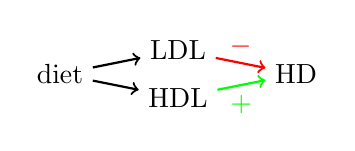
\begin{tikzpicture}
		\node (d1) at(0,0.0) {diet};
		\node (LDL) at(1.5,0.3) {LDL};
		\node (HDL) at(1.5,-0.3) {HDL};
		\node (HD) at(3,0) {HD};
		
		\draw[->,thick] (d1) -- (HDL);
		\draw[->,thick] (d1) -- (LDL);
		\draw[->,red,thick] (LDL) -- node[above,yshift=-1] {$-$} (HD);
		\draw[->,green,thick] (HDL) -- node[below] {$+$} (HD);
		\end{tikzpicture}
		\caption{}\label{fig:cholesterol:a}
	\end{subfigure}
	%
	\hfill
	%
	\begin{subfigure}{.45\linewidth}
		\center\
		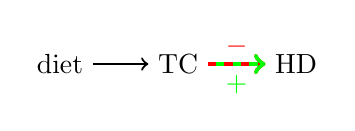
\begin{tikzpicture}
		\node (d1) at(0,0.) {diet};
		\node (LHDL) at(1.5,0) {TC};
		\node (HD) at(3,0) {HD};
		
		\draw[->,thick] (d1) -- (LHDL);
		\draw[->,red,dash pattern= on 3pt off 3pt,ultra thick] (LHDL) -- node[above,yshift=-1] {$-$} (HD);
		\draw[->,green,dash pattern= on 3pt off 3pt,dash phase=3pt,ultra thick] (LHDL) -- node[below] {$+$} (HD);
		\end{tikzpicture}
		\caption{}\label{fig:cholesterol:b}
	\end{subfigure}
	%
	\caption{Effects of cholesterol on risk of heart disease. As illustrated by~(a), the current consensus is that low-density lipoprotein (LDL) has a negative effect on heart disease (HD), while high-density lipoprotein (HDL) has a positive effect on heart disease. Considering total blood cholesterol (TC = LDL + HDL) to be a causal variable as in~(b) leads to problems: two diets promoting raised LDL levels and raised HDL levels respectively have the same effect on TC but opposite effects on heart disease. Hence different studies come to contradictory conclusions about the effect of TC on heart disease.}
	\label{fig:cholesterol}
\end{figure}


%In the following we give an example of the problems that can arise when there exists no consistent correspondence between two causal models, i.\,e.\ neither model can be viewed as an exact transformation of the other. This example falls into category (b) of the differing model levels listed above and was used by~\cite{spirtes2004causal} to illustrate problems in the causal modelling process.


Historically, the level of total blood cholesterol (TC) was thought to be an important variable in determining risk of heart disease (HD).
To investigate this, many experiments were carried out in which patients were assigned to different diets in order to raise or lower TC\@.
Conflicting evidence was found by these experiments: some found that higher TC had the effect of lowering HD, while others found the opposite \citep{truswell2010cholesterol,steinberg2011cholesterol}.

The reason for this apparent contradiction is clear with hindsight, but serves to illustrate the care that must be taken when seeking causal relations. 
The current scientific consensus is that there are two types of blood cholesterol, low-density lipoprotein (LDL) and high-density lipoprotein (HDL), which have a negative and positive effect on HD respectively (Figure \ref{fig:cholesterol:a}).
When measuring TC, the sum of LDL and HDL is measured.
Therefore two experiments, one raising LDL levels and the other raising HDL levels, would have the same effect on TC but opposite effects on HD (Figure \ref{fig:cholesterol:b}).

In this example, total blood cholesterol is too `coarse' a variable to have a well-defined causal relation with risk of heart disease. 
However, if it had been possible to affect only one of LDL and HDL through diet, this issue may never have been discovered:
if only HDL could be influenced by diet, the scientific consensus would be that total blood cholesterol is protective against heart disease and no contradictions would have been found.\footnote{Similarly, it is conceivable that there are in fact two different types of HDL: a more prevalent form which is protective against heart disease and one present in smaller quantities that has a detrimental impact. If the ratio of these two types is constant under any intervention through diet, the negative impact will always be outweighed by the positive impact and so we might never discover the detrimental subtype.}

This example raises two main points that we will discuss in the rest of this section. The first is that in the real world measurements or observations are always made at some level of detail or coarseness that is somewhat arbitrary. In the next subsection we will outline a variety of ways in which models of different levels of detail naturally arise in a variety of cases and further motivate the study of this fact in a causal setting.
The second is that whether or not a variable is `causally meaningful' is intricately connected to the interventions being considered. If we consider a coarse variable such as TC, we can consistently model causal relations if the interventions considered are sufficiently restricted, but this breaks down if the interventions are too rich. In subsection ?? we will discuss how to modify the framework of SEMs to take this into account.

The remainder of this section sets the stage for section ??, in which we tackle our overarching goal of trying to answer the following questions:
If the true causal mechanisms of the world operate at a very low level of detail (e.g. atoms), under what conditions can we speak of causal relations at higher levels (e.g. objects)?
How can we formalise such a notion of consistent modelling in the framework of SEMs?


\subsection{Modelling at different levels of detail}

Physical systems or processes in the real world are complex and can be understood at various levels of detail.
For instance, a gas in a volume consists of a large number of molecules.
But instead of modelling the motions of each particle individually (micro-level), we may choose to consider macroscopic properties of their motions such as temperature and pressure.
Our decision to use such macroscopic properties is first necessitated by practical considerations.
Indeed, for all but extremely simple cases, making a measurement of all the individual molecules is practically impossible and our resources insufficient for modelling the ${\sim}10^{22}$ particles present per litre of ideal gas.
Furthermore, the decision for a macroscopic description level is also a pragmatic one: if we only wish to reason about temperature and pressure, a model of $10^{22}$ particles is ill-suited.

Statistical physics explains how higher-level concepts such as temperature and pressure arise as statistical properties of a system of a large number of particles, justifying the use of a macro-level model as a useful transformation of the micro-level model~\citep{Balian}.
However, in many cases aggregate or indirect measurements of a complex system form the basis of a macroscopic description of the system, with little theory to explain whether this is justified or how the micro- and macro-descriptions stand in relation to each other.

Due to deliberate modelling choice or the limited ability to observe a system, differing levels of model descriptions are ubiquitous and occur, amongst possibly others, in the following three settings:

\begin{itemize}[noitemsep]
	\item[(a)] Models with large numbers of variables versus models in which the `irrelevant' or unobservable variables have been marginalised out \citep{bongers2016structural}; e.\,g.\ modelling blood cholesterol levels and risk of heart disease while ignoring other blood chemicals or external factors such as stress.
	
	\item[(b)] Micro-level models versus macro-level models in which the macro-variables are aggregate features of the micro-variables \citep{simon1961aggregation,iwasaki1994causality,hoel2013quantifying,chalupka2015visual,chalupka2016multi}; e.\,g.\ instead of modelling the brain as consisting of $100$ billion neurons it can be modelled as averaged neuronal activity in distinct functional brain regions.
	
	\item[(c)] Dynamical time series models versus models of their stationary behaviour \citep{fisher1970correspondence,iwasaki1994causality,dash2001caveats,lacerda2012discovering,mooij2013ode,mooij2013cyclic}; e.\,g.\ modelling only the final ratios of reactants and products of a time evolving chemical reaction.
\end{itemize}

%In the context of causal modelling, such differing model levels  should be consistent with one another in the sense that they agree in their predictions of the effects of interventions. The particular causal models we focus on in this paper are Structural Equation Models (SEMs, Section~\ref{sec:SEMs}, Section~\ref{sec:sem-for-causal-modelling}) \citep{spirtes2000causation,pearl2009causality}.
%
%In Section~\ref{sec:sem-transformation}, we introduce the notion of an exact transformation between two SEMs, providing us with a general framework to evaluate when two models can be thought of as causal descriptions of the same system.
%An important novel idea of this paper is to explicitly make use of a natural ordering on the set of interventions.
%On a high level, if an SEM can be viewed as an exact transformation of another SEM, we are provided with an explicit correspondence between the two models in such a way that causal reasoning on both levels is consistent.
%We discuss this notion of consistency in detail in Sections~\ref{subsec:causal-interpretation-transformation} and~\ref{sec:wrong}.
%
%In Section~\ref{sec:example-transformations} we apply this mathematical framework and prove the exactness of transformations belonging to each of the three categories listed above, with practical implications for the following questions in causal modelling:
%When can we model only a subsystem of a more complex system?
%When does a micro-level system admit a causal description in terms of macro-level features?
%How do cyclic SEMs arise?
%The fact that these distinct problems can all be considered using the language of transformations between SEMs demonstrates the generality of our approach.
%We close in Section~\ref{sec:questions} with a discussion.


%It is therefore not possible to transform the model in Figure~\ref{fig:cholesterol:b} into the model in Figure~\ref{fig:cholesterol:a} without leading to conflict:
%in order to reason about the causes of HD we need to consider the variables LDL and HDL separately.






\section{Transformations between Structural Equation Models}
\section{Examples of transformations}
\section{Discussion and work building on this}










































